

\section{The problem}

Imagine you have a big pot of money that you decide to lend out. There are two basic things you need to decide:

\begin{enumerate}
\item The maturity of the loans (how long you lend the money out for)
\item The riskiness of the borrowers
\end{enumerate}

The first is the \textbf{duration objective}, the second is the \textbf{credit objective}. Most  fixed income trading is in service of one of these. 

There are other important objectives such as exposure to particular currencies or inflation. These are important, but they are not core fixed income as they don't relate to the actual loans. 

Many different instruments and trading techniques are used to pursue these objectives. A major decision is whether to trade using \textbf{cash instruments} (claims to actual loans) or \textbf{derivatives} like forwards and swaps. Often the same objective can be pursued through both, but in different ways. There is a strong argument to use derivatives wherever possible, basically because it's cheaper.

The differences can be subtle and sometimes very difficult to quantify, largely due to the \textbf{non-linearities} inherent in fixed income instruments. This makes some aspects of fixed income trading more art than science. But it also makes it a richer and more textured landscape on which to paint the image of your portfolio preferences.

We'll proceed in four courses: first an aperitif of notation, and summaries of instruments, and processes; then a main course of duration and credit trading served with a side of popular carry and rolldown strategies. And for desert: inflation and currency.  If you're still hungry after that you might enjoy the appendix on credit instruments and pricing.


\section{Preliminaries}

\subsection{Notation}

\begin{itemize}
\item $AT$ - bond from issuer $A$ with maturity $T$
\item Zero coupon price: $P_{AT}^{FV}(t)$  -- price of a bond with a face value of \$FV from issuer $A$ with maturity $T$ at time $t$.
\item Zero coupon yield: $y(T1,T2)$  --yield on loan starting at $T1$ and maturing at $T2$ determined at $T1$
\item Zero coupon yield for a particular bond: $y_{AT}$ -- yield on the $AT$ bond
\item Zero coupon forward yield: $f(T1,T2)$ -- yield on loan starting at $T1$ and maturing at $T2$ determined now.
\item Swap: $SW_{AT_1,BT_2}$ -- self financed swap paying some amount of $AT_1$ and receiving one $AT_2$
\item Portfolio value: $V(t)$ -- value of some portfolio at time $t$
\end{itemize}

Unless otherwise specified all prices are for zero coupon bonds at $t=0$.

\subsection{Instruments}

\subsubsection{Bonds}

 A bond is a series of cashflows promised at different times in the future. A common structure is to have a final payment called the \textbf{face value} and regular payments called \textbf{coupons} as a percentage of face value. Some bonds have uncertain (\textbf{floating}) future payments. The price of a bond is the discounted value of all the payments.  Each payment should be discounted at the \textbf{zero coupon bond yield} for that maturity.

\subsubsection{Swaps}

A \textbf{swap} is any arrangement which swaps one series of cashflows for another. Since a series of cashflows is valued as a \textbf{bond}, a swap can be viewed as an exchange of bonds, or of a series of bonds. Often swaps are specified in terms of a \textbf{notional value}, with cashflows being either a \textbf{fixed rate} or a \textbf{floating rate} of the notional value with some regularity. For example a swap might swap the 3 month government rate for a fixed 4\% on a notional value of \$1M with payments each year. 


\subsubsection{Rates futures and forward rate agreements}
Bonds and swaps have a non-linear exposure to future interest rates. A \textbf{rate future} contract (sometimes called a \textbf{forward rate agreement}) is a linear exposure to rates at some point in future. For example a futures contract might be to pay \$100 times the three month interest rate in 9 months time. These provide a similar payoff to a certain type of interest rate swap, except that rates futures provide a payoff linear in the future rate where swaps are usually convex.

%For most simple bets on rates rate futures are an easy way to implement a particular view. For most of the examples below we won't use them because arbitrage the arbitrage argument is a little tricky. Using swaps gives us a clearer arbitrage argument so we can understand what's going on in the transaction. However for most purposes if you want to punt on interest rates or the shape of the curve rates futures are the way to go. 

\subsection{Processes}

\subsubsection{Repos}

It is possible to short sell bonds through \textbf{repurchase agreements} or \textbf{repos}. A repo is a borrowing agreement. We borrow a bond and agree to give it back later. Why do we do this? Because we immediately sell the bond for cash and \textbf{repurchase} it later when the loan is due.

If we have a riskless zero coupon bond with a face value of \$1 and two year maturity the short sale is like this:


\begin{center}
\begin{tabular}{|c|c|}
\hline
t=0 & Borrow bond \\
t=0 & Sell bond at market price for $P_{2}(0)$ cash  \\
       & (invest in a one year bond)\\
\hline
t=1 & Buy bond back at market price $P_2(1)$ \\
t=1 & Give bond back to lender\\
\hline
\end{tabular}
\end{center}

At $t=1$ the transaction is the risk free return on the repo cash less the cost to repurchase the bond: 

\[ V(1) =  \underbrace{P_2(0)\exp(y(0,1))}_{\textrm{risk free return}} - \underbrace{P_2(1)}_{\textrm{cost to repurchase loan}} \]

This generates the opposite return to short selling the one year bond to buy the two year bond. We do it to get a negative exposure to the price (and positive exposure to the yield). In this way we can use bonds to bet on future interest rates. The payoffs $V(1)$ as a function of price and yield is in figure \ref{fig:repo}.


\begin{figure}[ht]
\centering

\subfigure[As a function of price]{
   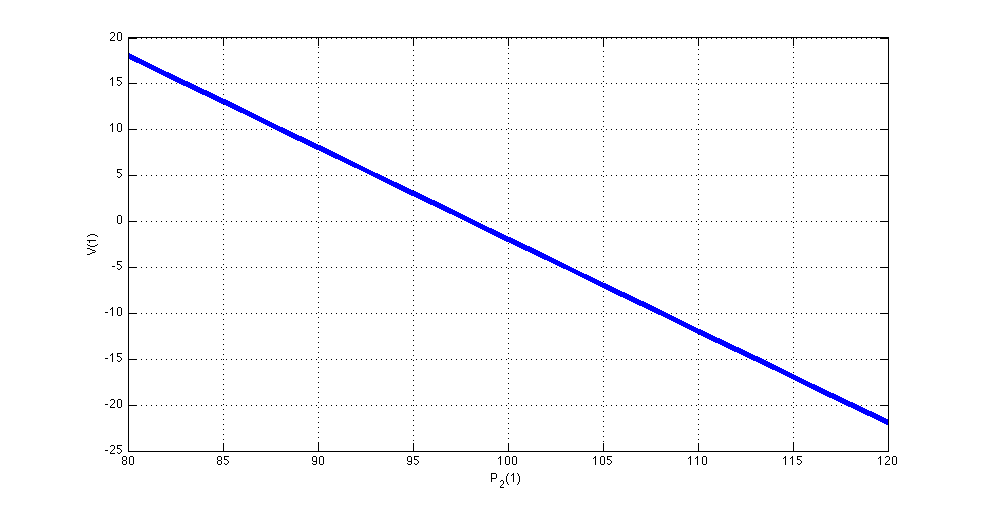
\includegraphics[width=3in] {pics/repoP}
   \label{fig:repoP}
 }

 \subfigure[As a function of future yield]{
   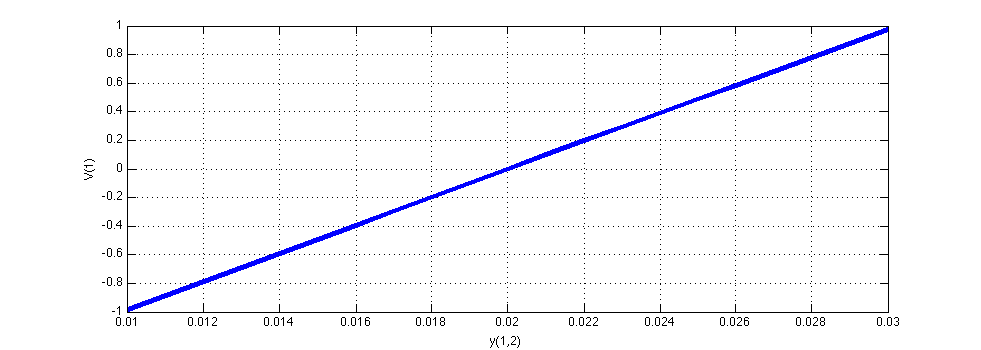
\includegraphics[width=3in] {pics/repoR}
   \label{fig:repoR}
 }
\caption{$V(1)$ for repurchase agreement}
\label{fig:repo}
\end{figure}


%set asset repo as exercise. 
 
%There's a deeper point here. All assets are bought with other assets and so all yields must be contrasted with the yields of alternative assets. This is visible when we do a short sale because we have to reacquire the repo at a different price, but it is nonetheless a real cost. If I borrow (short sell) money to buy a house I want the house to appreciate more than a money asset.\footnote{adjusted for the value the house provides} But if I start with \$100 and leave it in cash I am still \textit{short} houses even though I don't have a repurchase agreement.

%We've assumed that the bond is riskless so why would anybody be willing to loan the bond to you or me for no extra? It's true that they end up in the same position but that's only if we don't scamper off with the bond. In the real world repos are costly but not as much as you would think.

Aren't we forgetting something? Shouldn't there be an interest rate on the repo? The surprising answer is ``no".  The reason is that whoever lends the bond doesn't lose anything provided that the bond is repaid. Since they don't lose anything they should be satisfied with a token payment close to zero for the loan plus something for the credit risk. The credit risk approaches zero if the contract has sufficient collateral and is well margined.

\subsubsection{Collateral and margining} 

The easiest way to reduce credit risk on a repo is to provide a large amount of collateral. If there is a sufficiently large buffer between the value of the loan and the saleable value of the collateral the loan becomes riskless.

Home loans are a good example. A home loan is a repo (short selling a bond) and a long position in an asset. The loan (repo) is collateralised with the asset: if you stop paying your mortgage the bank will sell your house. If the value of the house is always more than the value of the loan they can't lose. The same principle applies to other repos. If you provide a sufficiently valuable asset as collateral the repo rate will approach zero.\footnote{This isn't true if the asset pays any income like coupons or dividends over the course of the repo. If it does the repo rate will include the discounted value of these payments.}

A clever technique for collateralising a repo is \textbf{margining}. Margining is when you give a little bit of collateral initially but demand more (in a \textbf{margin call}) if the asset price moves adversely. If the price changes are small relative to the margin there's no credit risk because the contract can be closed if fail to pay a margin call. 

\textbf{Example: margining}
Say I enter a futures contract to buy a tonne of corn in a year's time for \$100. I put up 10\% of the price as margin.  The futures price moves to \$105 so I have to provide an additional \$5 in margin to keep the 10\% buffer. If I don't provide the margin the futures seller closes out the contract an reenters with another buyer. As long as the margin is large enough to cover market moves there is no credit risk. After a year the contract can settle in cash because the accumulated margins will equal the difference between the contracted futures price and the spot price at expiry.

\subsubsection{Self financed portfolios}

Say you have two zero coupon bonds: $AT_1$ and $BT_2$. We can construct a portfolio by repoing (short selling) a certain amount of the first bond to finance the purchase of one of the second bond. 

To buy one $BT_2$ we need to repo  $P_{BT_2}(0)/P_{AT_1}(0)$ of the $AT_1$s. The total portfolio value is

\[V(0) =  -\frac{P_{BT_2}(0)}{P_{AT_1}(0)}*P_{AT_1}(0) + P_{BT_2}(0) = 0 \]

after $T1<T2$ the value first bond has matured and repays FV (face value) so the value is

\[V(T1) = -\frac{P_{BT_2}(0)}{P_{A_T1}(0)}*FV + P_{BT_2}(T1)   \]

If the face value is a constant the only uncertain value is $P_{BT_2}(T1)$. In summary this portfolio costs zero upfront and is a linear bet on the future value of $P_{BT_2}(T1)$ (and a non-linear bet on the future yield $y_B(T_1,T_2)$)

 
\subsection{Pricing and sensitivities}

The value of a series of payments is the sum of the discounted values of each payment. The sensitivity of the value is given by the derivatives of the value function.

\subsubsection*{Price:} For some set of cashflows  $(C1, C2,\ldots ,CN)$ received from borrower $A$ at times  $(T_1, T_2,\ldots ,T_N)$ the value is 
\[V(C1, C2,\ldots ,CN) = C1\exp(-y_{AT_1}*T_1) + C2\exp(-y_{AT_2}*T_2) +  \ldots + CN\exp(-y_{AT_N}*T_N)\]

\subsubsection*{Dollar yield:} The dollar yield of the portfolio is change in value over time:

\begin{eqnarray*}
\frac{\partial V}{\partial t} &= y_{AT_1}C1P_{AT_1}^1 + y_{AT_2}C2P_{AT_2}^1+  \ldots + y_{AT_N}CNP_{AT_N}^1 \\
 &= y_{AT_1}C1\exp(-y_{AT_1}*T_1) + y_{AT_2}C2\exp(-y_{AT_2}*T_2) +  \ldots + y_{AT_N}CN\exp(-y_{AT_N}*T_N)
\end{eqnarray*}

\subsubsection*{Dollar duration:} The duration is the change in value with parallel shift in all yields on the curve (the common component of yields is denoted $\bar{y}$):

\begin{eqnarray*}
\frac{\partial V}{\partial \bar{y}} &= -T_1C1P_{AT_1}^1 - T_2C2P_{AT_2}^1 -  \ldots - T_NCNP_{AT_N}^1\\
 &=   -T_1C1\exp(-y_{AT_1}*T_1) - T_2C2\exp(-y_{AT_2}*T_2) -  \ldots - T_NCN\exp(-y_{AT_N}*T_N)
\end{eqnarray*}

\subsubsection*{DV01:} The duration expressed as a response for a 0.0001 change in yield:

\[ DV01 =  \frac{\partial V}{\partial \bar{y}}/10000\]

For a zero coupon bond with a face value of \$100, a yield of $y$ and maturity $T$ we have

\begin{itemize}
\item[] \textbf{Price of a zero coupon bond:} $P = 100*exp(-y*T)$\\
\item[] \textbf{DV01 (sensitivity to a 1bp change in yield):} $DV01 = -T*P/10000$\\
\item[] \textbf{Dollar yield (sensitivity to change in time):} $DVT = y*P$
\end{itemize}


\section{Duration and credit}

\subsection{Jesus and Shifty Steve}

Imagine a very simple fixed income market with two borrowers: \textbf{Jesus} and \textbf{Shifty Steve}. Jesus is a very reliable debtor (and a great guy!). He always repays his debts. Shifty Steve is less reliable. Both debtors borrow a large amount of money for one and ten years and these loans (which are zero coupon bonds) can be bought and sold in arbitrary quantities. No other loans exist. 

On the day we observe the market  the yields and prices for \$100 of face value as follows:

\begin{center}
\begin{tabular}{|c|cc|cc|}
\hline
 & 1 year yield & 1 year price & 10 year yield & 10 year price\\
 \hline
 Jesus & 1\%  &  \$99.01 & 1.5\% & \$86.07\\
 Steve & 2\% & \$98.02 & 6\%  & \$54.88\\
 \hline
 \end{tabular}
 \end{center}

We will explore the duration and credit decisions by examining these loans. We'll assume (unrealistically) that we can buy and sell all bonds costlessly and that there is no cost for repos. For the repos the alternative asset must be one of these four bonds: If I want to short 10 year Jesus bonds I'll need to buy some amount of the other three . 

\subsection{The duration objective}

The first thing to note is that 10 year bonds are much more sensitive to movements in interest rates than one year bonds. If the 1 year rate increases by 1\% the J1 goes from 99.01 to 98.02. If the 10 year rate increases by 1\% the J10 goes from 86.07 to 77.88. This is because the 10 year bond has a much higher duration (10 times higher). The dollar duration, or DV01, is the sensitivity of a bond to a one basis point (1/100 of a percent) increase in yields. These are:


\begin{center}
\begin{tabular}{|c|c|c|}
\hline
 & 1 year DV01 & 10 year DV01\\
 \hline
 Jesus & $DV01_{J1} = 1*J1/10000 = .009901$  & $DV01_{J10} = 10*J10/10000 =  .08607$\\
 Steve & $DV01_{S1} = 1*S1/10000 = .009802$  & $DV01_{S10} =10*S10/10000 = .05488$\\
 \hline
 \end{tabular}
 \end{center}

\textbf{A fully financed Jesus portfolio}\\
Focus just on Jesus first.  If we want to buy \$100 worth of 10 year bonds we have to (short) sell \$100 worth of 1 year bonds. The ratio of exchange between the two bonds is the ratio of price: 86.07/99.01 = 0.87. So we have to sell 0.87 J1s to get a J10. 

The current value of the portfolio is:

\[V(0) = -0.87*P_{J1}(0)+P_{J10}(0) = 0 \]

And after one year:

\[V(1) = -0.87*100 + P_{J10}(1)  \]

The annualised yield (in dollars) is

\[\frac{\partial V}{\partial t} = -y_{J1}*0.87*P_{J1}+y_{J10}P_{J10} = 0.4303  \]

So the annualised return on the portfolio is currently \$0.4303. 

The portfolio has a dollar duration (DV01) of 

\[ \frac{\partial V}{\partial \bar{y} }/10000= -0.87*DV01_{J1}+1*DV01_{J10} = 0.0775  \]

Which means that a one basis point increase in both 1 and 10 year yields will cost approximately \$0.0775. This is only approximate because both bonds have convexity (the sensitivity changes with the yield). %We can get a better estimate by using a Taylor series approximation. 

\textbf{A swap representation}\\
A useful way to view this transaction is as a swap. The swap is entered at $t=0$ and at time $t=1$ pays 0.87 J1's and receives 1 J10 (see figure \ref{fig:durationSwap})

\begin{figure}[ht]
\centering
  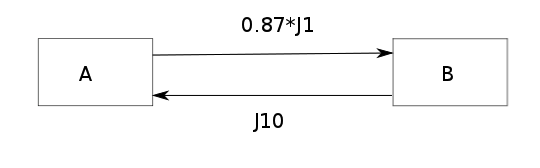
\includegraphics[width=5in] {pics/durationSwap}
\caption{$SW_{J1,J10}$ swap}
\label{fig:durationSwap}
\end{figure}

%I'm agreeing that in a year from now I'll pay $x$ J1s and receive a J10 (which will then be a J9 with price $100exp(-f(1,10))$ where $f(1,10)$ is the forward rate calculated as

%\[y_J(1,10) = \frac{10*y_J(0,10)-1*y_J(0,1)}{10-1} = \frac{10*0.015 - 0.01}{9} = 0.0156 \]

%(Remember that this forward rate exists by arbitrage) To make the swap have a zero net present value we solve

%\begin{eqnarray*}
%x*100*exp(-y_J(0,1)) = 100*exp(-y_J(1,10)*9)*exp(-y_J(0,1)) \\ 
%\Rightarrow x \approx 0.87
%\end{eqnarray*} 

We assume that the swaps are available in unlimited quantities. We'll call the swap $SW_{J1,J10}$ for short. Dealing with the swap directly makes things a lot more clear: it is  a bet on interest rates. Specifically it is a bet that in a year's time the yield of a J10 with 9 years left to maturity will be less than the forward rate 1.56\%. This is the rate for the J10 that makes V(1)=0. The payoff diagram is in figure \ref{fig:swap}. Notice that the payoff is slightly non-linear as a result of the non-linearity of the underlying bond.

\begin{figure}[ht]
\centering

\subfigure[As a function of price]{
   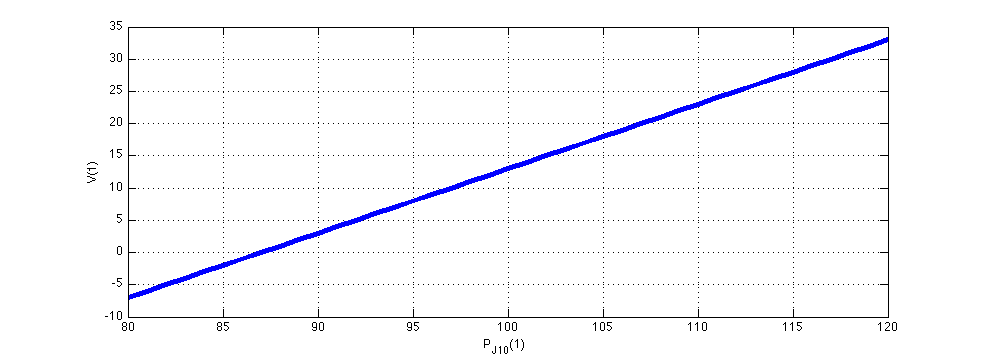
\includegraphics[width=3in] {pics/durationSwapP}
   \label{fig:durationSwapP}
 }

 \subfigure[As a function of future yield]{
   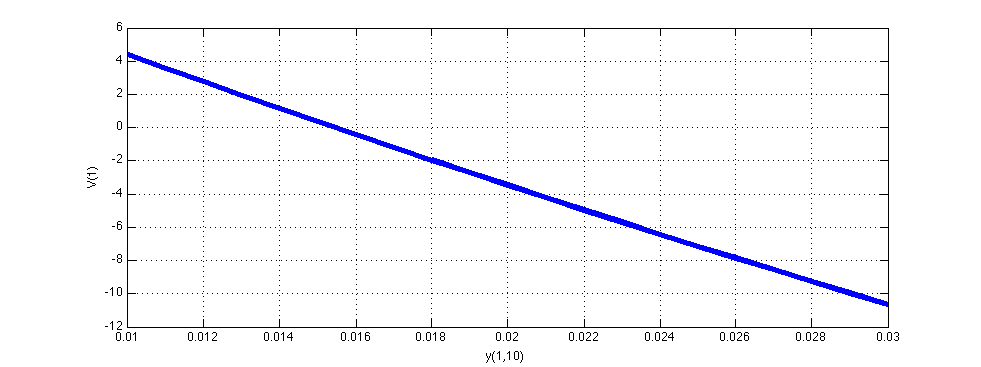
\includegraphics[width=3in] {pics/durationSwapR}
   \label{fig:durationSwapR}
 }
\caption{$V(1)$ for swap}
\label{fig:swap}
\end{figure}

\subsection{The credit objective}

We just used a swap to manufacture a pure bet on risk free interest rates. We can do a similar thing to manufacture a bet on whether Steve will repay his loan. Such a swap serves a useful purpose since the only reason anybody would lend to Steve rather than Jesus is the higher yield he pays on the bond. It's convenient to bet on Steve's creditworthiness directly.  Don't get too excited yet, but we're about to make a Credit Default Swap.

\textbf{A Jesus financed Steve portfolio}\\

We can buy an S1 by short selling 98.02/99.01 = 0.99 J1s. After a year we pay 100*0.99 = \$99 on our short Jesus and receive some amount (hopefully \$100) from Steve. But we might not get the whole \$100 from Steve. He's a shifty character, and there's a possibility he'll repay some lesser proportion $R$ of the \$100 when the bond comes to maturity. 

The current value of the portfolio is:

\[V(0) = -0.99*P_{J1}(0)+P_{S1}(0) = 0 \]

And after one year:

\[V(1) = -0.99*100 + P_{S1}(1)  = -99+ R*100 \]

The yield (in dollars) is

\[ \frac{\partial V}{\partial t}  = -y_{J1}*0.99*P_{J1}+y_{S1}P_{S1} = 0.9802 \]

So the current yield is around \$0.98 per year.

The portfolio has a dollar duration (DV01) of 

\[ \frac{\partial V}{\partial \bar{y}} =  -0.99*DV01_{J1}+1*DV01_{S1} = 0  \]
 
Which means that a one basis point increase in both Jesus and Steve's one year rate will have close to no effect (the sensitivity is zero, but the pricing function is convex so the effect isn't exactly zero). What matters in this transaction is the \textit{difference} between the  two rates, and ultimately the difference between the money you pay to cover the short Jesus and the amount you get back from Steve. Some people like to create a sensitivity measure called \textbf{spread duration} that gives the DV01 sensitivity of a portfolio to changes in the yield spread between the two bonds.  We can see better if we specify the yield on the S1 as the yield on the J1 plus a spread, then:

\begin{eqnarray*}
V(0) &= -0.99*P_{J1}(0) + P_{S1}(0)\\
 &= -0.99*100*\exp(-y_J(0,1))+100*\exp(-(y_J(0,1)+S)) 
 \end{eqnarray*}

Where $S$ is the spread (1\%). 

The spread duration is just the yield sensitivity on the S1:

\[ \frac{\partial V}{\partial S} = T *100*\exp(-(y_J(0,1)+S)) = 1*100*(\exp(-0.02*1)) = 0.0098 \]

So each 1bp increase in the spread costs the swap \$0.0098.

\textbf{A credit default swap representation}\\

This arrangement described is a swap. After one year the swap pays 0.99 J1s  and receives an S1. By assumption $P_{J1}(1) = 100$ and $P_{S1}(1) = 100*R$. This is a kind of \textbf{credit default swap} because the future value depends on the amount of the default. The swap is in figure \ref{fig:creditSwap}, the payoff profile after a year is in figure \ref{fig:CDSR}.

\begin{figure}[ht]
\centering
  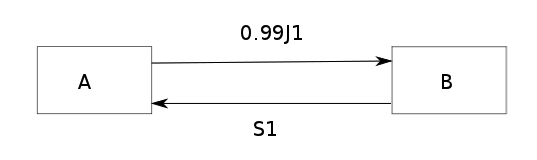
\includegraphics[width=5in] {pics/creditSwap}
\caption{$SW_{J1,S1}$ swap}
\label{fig:creditSwap}
\end{figure}

\begin{figure}[ht]
\centering
  \includegraphics[width=5in] {pics/CDSR}
\caption{$V(1)$ for CDS as a function of repayment rate}
\label{fig:CDSR}
\end{figure}

We'll call this swap $SW_{J1,S1}$. You can think of the 0.99 as the swap rate. It's a convenient way to bet Steve's credit worthiness without having to put up any cash up front.

This is a \textit{kind} of credit default swap but usually these are specified differently. Usually a CDS pays a certain amount now for protection against default later. The up front price is just the difference between the two bonds: S1-J1 = 99.02-98.01 = 1.01. It has to be because holding the swap \textit{and} an S01 gives the same payoff as a J01. 

The character of two remaining swaps $SW_{S1,J10}$ and $SW_{S1,S10}$ is left as an exercise.

\subsection{Summary}

\textbf{The duration objective}:\\
To trade the forward rate between $T_1$ and $T_2$ ($T_1<T_2$) for a risk free borrower $A$:
\begin{itemize}
\item Short sell $P_{AT_2}(0)/P_{AT_1}(0)$ of the $AT_1$s\\
\item Buy one of the $AT_2$s
\end{itemize}

At $t=0$ this portfolio has zero value. At $t=T_1$

\[V(T_1) = -\frac{P_{AT_2}(0)}{P_{AT_1}(0)}P_{AT_1}(T_1) + P_{AT_2}(T_1)   \]

The only uncertain variable is the $P_{AT_2}(t)$ price. This depends on the prevailing yield at $t=T1$. The breakeven for this trade is at the forward rate $f_A(T_1,T_2)$. The process is encapsulated in the \textbf{swap} $SW_{AT_1,AT_2}$

\textbf{The credit objective}:\\
To trade the credit of some risky borrower $B$ at a maturity $T$:

\begin{itemize}
\item Short sell $P_{BT}(0)/P_{AT}(0)$ of the $AT$s (the risk free bond)\\
\item Buy one of the $BT$s (the risky bond)
\end{itemize}

At $t=0$ the portfolio has zero value. At $t=T$

\[ V(T) = \frac{P_{BT}(0)}{P_{AT}(0)}P_{AT}(T) + P_{BT}(T) \]

The price of $AT$ is guaranteed since the bond is risk free, the price of $BT$ is linear in the recovery rate on the bond $R$. The process is encapsulated in a \textbf{credit default swap} $SW_{AT,BT}$.


\section{Trading}

A fixed income trader has two related tasks: 

\begin{enumerate}
\item Construct forecasts of future interest and repayment rates.\\
\item Construct a combination of trades to create a desired portfolio
\end{enumerate}

The first task is tricky.  A set of arbitrage free prices gives us almost no useful information. We can know the risk neutral expectations, -- the forward rates and forward spreads -- but those are the rates that give us zero profit. To forecast we have to bring some insight from outside. This might be some unexploited statistical regularity, or some superior understanding of the operation of a particular market.  These things are outside the scope of this chapter. Here we will focus on the second task. 

Swaps are a more direct way to bet on future interest rates and default rates than investing in bonds separately. It is almost always best to hold the minimum number of cash bonds in a portfolio. Most fixed income funds have the majority of their money in very short term securities with a collection of swaps (and other more exotic things) to transform the yield curve and credit exposure. It is common for a particular bond to trade thinly or not at all while a swap that creates the same exposure is highly liquid. 

In this section we'll demonstrate a few techniques for constructing trades.

\subsection{Hitting yield and DV01 targets}

The job of a fixed income trader is to construct a portfolio with some desirable characteristics. For example a client might want an unfunded portfolio to yield \$10 a year, with a spread duration of precisely \$0.05. Since portfolios sensitivities are linear in the instruments this is easy to do. 

If we just wanted to get to \$10 yield we could do it with both swaps from the previous section.  The $SW_{J1,J10}$ has a \$0.403 yield so we need $10/0.403 = 23.24$ times the exposure of the swap to get to \$10.  Increasing the exposure means increasing the notional value. If we increase the \textbf{notional value} by 23.24 times  from \$100 to \$2324 on the $J10$ leg of the swap. The $SW_{J1,S1}$ has  a yield of \$0.9802 so we need $10/0.9202 = 10.20$ times the exposure on the $S1$ leg -- a notional value of \$1020. 

\begin{tabular}{|c|ccccc|}
\hline
 & $J1$ face value & $J10$ face value & $S1$ face value & Yield & Spread duration\\
\hline
$SW_{J1,J10}$ & -87 & 100 & 0 & 0.403 & 0\\
$SW_{J1,S1}$ & -99 &  0 & 100 &  0.9802 & 0.0098\\
\hline
\end{tabular}

The spread duration of a \$100 notional value $S_{J1,S1}$ is 0.0098 so we'll need $0.05/0.0098 = 5.10$ times the exposure (\$510 notional value). This gives a yield of \$5 so we need to get the other \$5 of yield from 100*5/0.4303 = \$1162 notional value in the $SW_{J1,J10}$ swap.

One way to view these type of problems is as a set of linear constraints. Figure \ref{fig:yieldDV01} has the combinations of notional values required to hit the yield (blue line) and spread duration (red line) constraints. Each extra restriction is a line in this space. For simple problems this can be viewed graphically, more complicated problems can be solved with straightforward linear programming techniques (or if you're lucky just by solving a set  of linear equations). 

\begin{figure}[ht]
\centering
  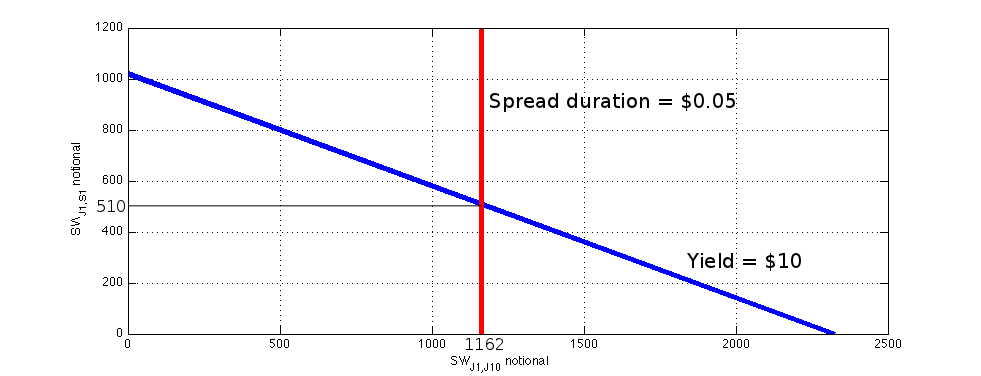
\includegraphics[width=5in] {pics/yieldDV01}
\caption{Notional swap value combinations to hit DV01 and yield targets}
\label{fig:yieldDV01}
\end{figure}

\subsection{Trading the curve}

We've constructed trades to have exposure to a particular forward rate. It's also possible to construct trades that have exposure to more than one forward rate. These combination trades allow traders to express more general views. For example it's possible to construct a trade to bet that the future yield curve will be \textbf{steeper or flatter} than the current forward curve suggests. It's also possible to construct a trade that the curve will be \textbf{more or less convex}.

We'll do this all with swaps. To give a bit more texture to the example we'll add a two more maturities for the Jesus bonds. The zero coupon yields and the nearby forward yield is in the table below.

\begin{center}
\begin{tabular}{|c|ccccc|}
\hline
Maturity & 1 & 2 & 3 & 5 & 10\\
Yield & 1\% & 1.056\% & 1.111\%& 1.22\% & 1.5\%\\
Forward &  & f(1,2) = 1.11\% & f(1,3) =1.167 & f(1,5) = 1.28\% & f(1,10) = 1.56\%\\
\hline
\end{tabular}
\end{center}

The swaps paying the one year bond  are $SW_{J1,J2}$, $SW_{J1,J3}$, $SW_{J1,J5}$, and $SW_{J1,J10}$. Each swap has final payoff that depends on one of the three forward rates. We'll calculate the DV01 in terms of these forward rates, and a reciprocal which is the notional value of the swap (on the receive side) that gives \$1 in DV01 to the forward rate. 


\begin{center}
\begin{tabular}{|c|c|c|c|}
\hline
Swap & Forward rate & DV01 to forward rate at $t=1$ & notional per \$1 of DV01\\
\hline
$SW_{J1,J2}$  & f(1,2) & $1*100*\exp(f(1,2)*1)/10000 = 0.0101$ & 100/0.0101 = 9889.5\\ 
$SW_{J1,J3}$  & f(1,3) & $2*100*\exp(f(1,3)*2)/10000 = 0.0205$ & 100/0.0205 = 4884.7\\ 
$SW_{J1,J5} $ & f(1,5) & $4*100*\exp(f(1,5)*4)/10000 = 0.0405$ & 100/0.0405 = 2468.3\\ 
$SW_{J1,J10}$  & f(1,10) & $9*100*\exp(f(1,10)*9)/10000 = 0.0914$ & 100/0.0914 = 1094\\ 
\hline
\end{tabular}
\end{center}

We'll also need the notional value of the underlying bonds and the dollar yields:

\begin{center}
\begin{tabular}{|c|ccc|}
\hline
Swap & $J1$ face value & Receive face value & Yield  \\
\hline
$SW_{J1,J2}$  & 97.91 & 100  & 0.5483  \\ 
$SW_{J1,J3}$  & 96.72  & 100  & 0.1064   \\ 
$SW_{J1,J5} $ & 95.08  & 100  & 0.207  \\ 
$SW_{J1,J10}$  & 86.07 &  100 &0.4304  \\ 
\hline
\end{tabular}
\end{center}

Now we're ready to trade the curve!

\subsubsection{Trading the level}

Say we believe that the forward curve will be uniformly higher across all maturities at $t=1$. Since the swaps have a negative exposure to the rate we'll need to sell swap (pay the long rate, receive the short rate). We can trade this with any of the three swaps in proportion to their DV01. To get the same exposure the $SW_{J1,J5}$ needs 2468.3/1094 = 2.25 times the exposure of the $SW_{J1,J10}$; or 9889.5/1094 = 9.04 times the exposure of the $SW_{J1,J2}$.

The picture is figure \ref{fig:level}.

\begin{figure}[ht]
\centering
  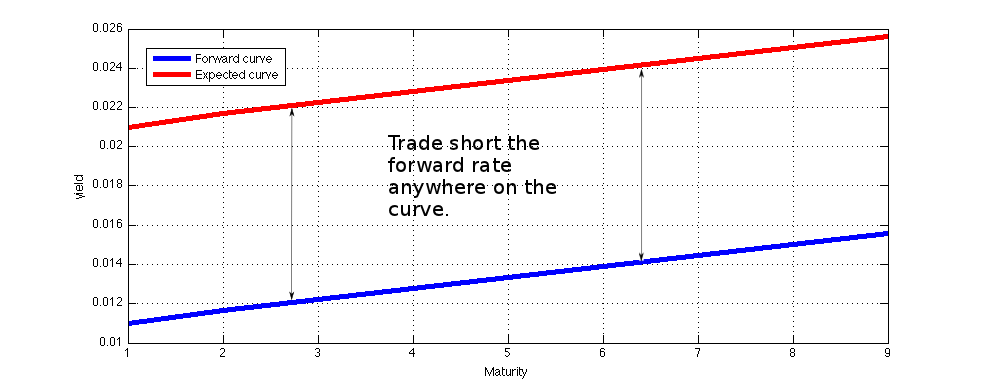
\includegraphics[width=5in] {pics/level}
\caption{Forward curve against expected future spot curve}
\label{fig:level}
\end{figure}

\subsubsection{Trading the slope: steepeners and flatteners}

Say we believe that the future yield curve will be steeper than the forward curve. We can trade this by buying the $SW_{J1,J2}$ and selling the $SW_{J1,J10}$ in proportion to their DV01s. To get \$1 of exposure each side we need \$9889.5 of notional from the $SW_{J1,J2}$ and \$1094 of notional from the $SW_{J1,J10}$. The trade will make more money if the future curve is steeper than the forward curve. This trade, and trades with the same effect, are called \textbf{steepeners}.

If we believe the future curve will be flatter we can do the opposite trade. Then it is called a \textbf{flattener}.

Notice that the level of the curve doesn't affect the trade (except a little through convexity). The curve could end up entirely above or below the current forward curve and the trade would still have the same (approximate) effect. All that matters is the slope of the curve between the 4 and 9 year maturities.  Note also that the trade is \textbf{duration neutral}. The picture is figure \ref{fig:slopes}.

\begin{figure}[ht]
\centering

\subfigure[Steepener]{
   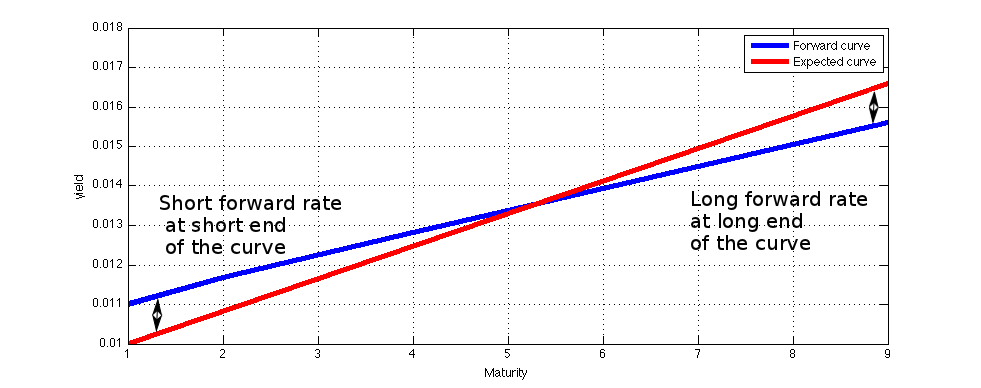
\includegraphics[width=3in] {pics/steepener}
   \label{fig:steepener}
 }

 \subfigure[Flattener]{
   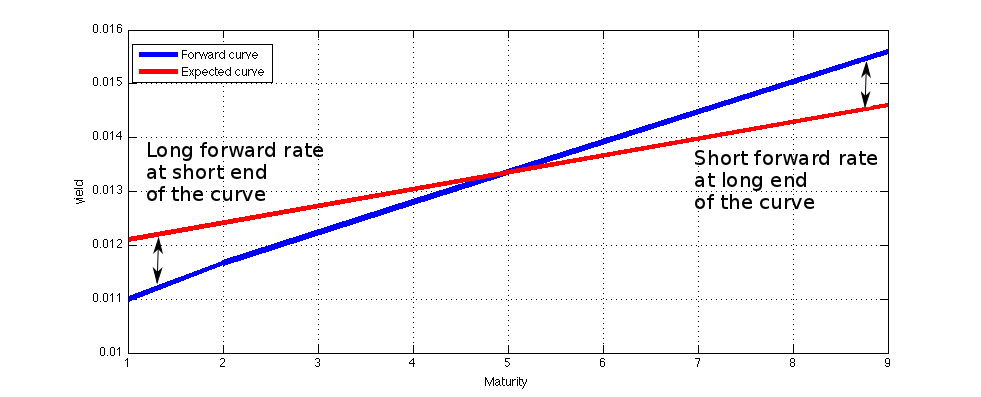
\includegraphics[width=3in] {pics/flattener}
   \label{fig:flattener}
 }
\caption{Curve slope trades}
\label{fig:slopes}
\end{figure}

\subsubsection{Trading convexity}

Supposing instead we thought the future curve would be more convex than the forward curve. In our example the forward curve is linear so any convexity will do. A convexity trade requires three points on the curve: one long rate, one short rate, and one middle rate. Our belief in future convexity of the curve means we think the curve will bend inwards, with the long and short rate decreasing by more than the middle rate (see picture). For this we buy DV01 adjusted amounts of $SW_{J1,J2}$ and $SW_{J1,J10}$ and sell \textit{twice} as much DV01 adjusted $SW_{J1,J5}$ to make the trade duration neutral.

This trade is commonly called a \textbf{butterfly} (the long and short rate trades are the `wings' of the insect, the middle rate trade is the body). We could also do the trade in reverse if we thought the future curve would be less convex than the forward curve. The picture is figure \ref{fig:butterfly}.

\begin{figure}[ht]
\centering
  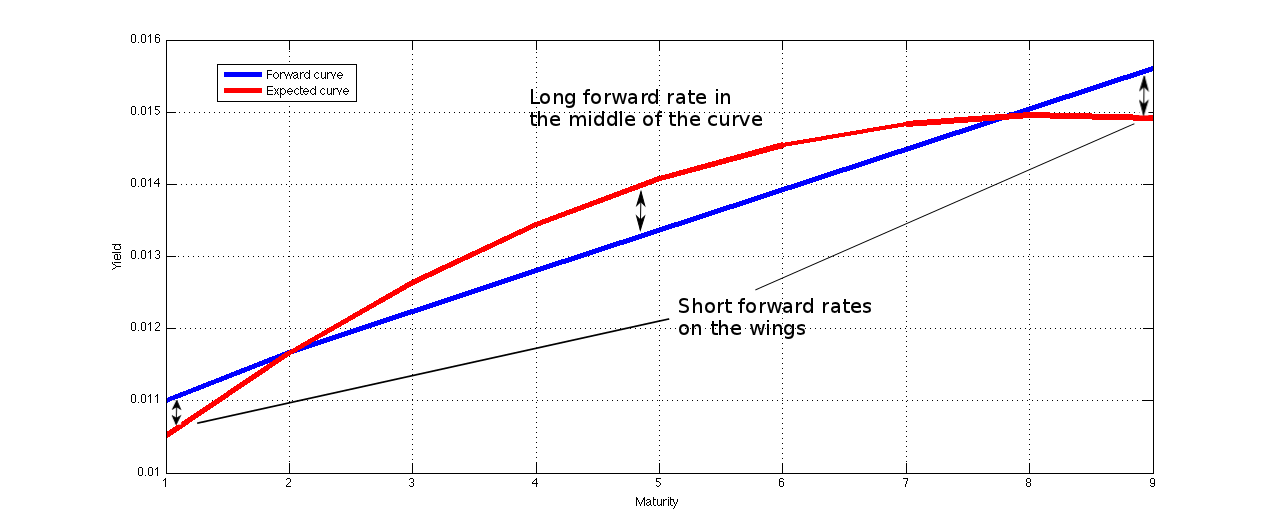
\includegraphics[width=5in] {pics/butterfly}
\caption{Butterfly}
\label{fig:butterfly}
\end{figure}

\subsection{Trading credit}

Trading credit is similar to trading rates. A credit trade is a bet on the future market expectation of default. If a company actually defaults there is usually still some uncertainty over how much a sale of assets will return bondholders.  For each borrower there is a curve giving the spread against a less risky bond (usually the government curve). This curve can be traded in the same way as rates: with steepeners and flatteners and butterflies and such.

To trade the possibility of default directly we can trade either $SW_{J1,S1}$ or $SW_{J10,S10}$. Both give a direct exposure to the default rate at $t=1$ and $t=10$. Trading $SW_{J1,S10}$ gives an exposure to the nine year \textbf{forward rate} on the S10 one year forward.

Individual CDSs often have a large \textbf{bid offer spread} because the underlying bonds are difficult to buy and sell. This leads many to trade \textbf{credit default swap indices} based on the \textbf{credit spread} of a number of different entities. There are different indices for different credit classes, as well as for geographical and industry groupings. There are a number of other widely traded credit derivatives: \textbf{Collateralised Debt Obligations} (CDOs) are instruments that take some portion of the credit exposure from a bond, or from a collection of bonds. There are also options on bonds, rates (caps/floors), and swaps (swaptions), and an endless rainbow of exotic derivatives. 

There is a lot more to say about  credit instruments and trading, but we'll leave the discussion to the discussion on credit.

\subsection{Hedging interest rate risk}

Fixed income trading isn't all punting on rates and spreads. There is the occasional legitimate hedger. Businesses wish to remove interest rate risk, either from existing floating rate loans, or for future loans they intend to make or receive. This hedging can be done in (at least) two ways: either with swaps for each uncertain payment, or a single swap on all uncertain payments.

In both cases the swap is priced by finding  a fixed rate that makes the fixed and floating legs of the swap equal discounted values. Uncertain future rates are evaluated at the forward values (e.g. $y(2,3)$ is given the value $f(2,3)$).

%as a trade on a single future rate, or on a series of rates. If the business already has a floating rate loan, it's a simple matter to create a fixed-for-floating swap to remove the uncertainty associated with the future interest rate rises. Each uncertain future rate has a market determined forward rate, a \textbf{fixed for floating swap} replaces regular uncertain (floating) payments by regular fixed payments. The fixed rate is the rate that makes the present value of all floating payments evaluated at the appropriate forward rate equal to the present value of the fixed payments. 

\subsubsection*{Example: Hedging with multiple swaps}
Say that you are short a bond with a \$100 face value with a \textbf{floating coupon} equal to the Jesus rate (risk free) + 2\%. The bond maturity is 2 years, and coupons are paid annually. You are exposed to the risk that the Jesus rate will increase. 

For the first payment the swap rate is the forward value of the payments, which is the forward rate plus 2\%:

\begin{center}
\begin{tabular}{|ccc|}
\hline
Time & floating payment & fixed payment\\
\hline
1 & $100*(y_J(1,2)+0.02)$ &  $100*F_1$\\
\hline
\end{tabular}
\end{center}

The swap rate is $F_1 = f(1,2)+0.02 =$ 3.11\%.

Similarly for the second payment:

\begin{center}
\begin{tabular}{|ccc|}
\hline
Time & floating payment & fixed payment\\
\hline
2 & $100*(y_J(2,3)+0.02) + 100$ & $100*F_2 + 100$\\
\hline
\end{tabular}
\end{center}

The swap rate is $F_2 = f(2,3) + 0.02 =$ 3.22\% 


%To hedge this risk you can enter into two \textbf{forward rate agreements}, one for each coupon. These agreements specify that you can borrow at a future point in time for a fixed rate. These will each be priced at the forward rates $y(1,2) = 1.11\% $ and $y(2,3) = 1.22\%$. With these FRA's in your top drawer you are guaranteed to pay in net 1.11+2 = 3.11\% for the first coupon and 1.22+2 = 3.22\% for the second coupon. WRONG BECAUSE FRA IS LINEAR 

\subsubsection*{Example: Hedging with a single swap}
We can also hedge out the risk with a swap which pays a fixed coupon and receives the floating rate. The swap payments look like this (we'll call the fixed rate $F$):

\begin{center}
\begin{tabular}{|ccc|}
\hline
Time & floating payment & fixed payment\\
\hline
0 &  & \\
1 & $100*(y_J(1,2)+0.02)$ &  $100*F$\\
2 & $100*(y_J(2,3)+0.02) + 100$ & $100*F + 100$\\
\hline
\end{tabular}
\end{center}

To get the swap rate we make the discounted values of these payments equal, with the uncertain future rates evaluated at the forward rates.

\begin{eqnarray*}
V(0) = \exp(-y(0,1)*1)*100*(f(1,2)+0.02) + \exp(-y(0,2)*2)*(100*(f(2,3)+0.02) +100) \\
- (\exp(-y(0,1)*1)*100*F + \exp(-y(0,2)*2)*(100*F+100))  = 0
\end{eqnarray*}

Which gives $F=3.1647\%$. By entering into the swap you remove the interest rate risk. You still pay the floating rate on the bond but the swap pays the difference between the floating coupon and the fixed swap rate.


\subsection{Summary}

Trading is mostly about constructing portfolios to do certain things: to hit sensitivity targets and/or to have an exposure to the forward curve. Hitting sensitivity targets is easy since bond and swap portfolios are linear in sensitivities. Constructing exposures to the forward curve is easy with swaps since swaps can be constructed to have a breakeven at any desired forward rate.

To get exposure to the a risk free forward rate $f_A(T_1,T_2)$ trade the swap $SW_{AT_1,AT_2}$ since this has

\[V(0) = \frac{-P_{AT_2}(0)}{P_{AT_1}(0)}P_{AT_1}(0) +  P_{AT_2}(0) = 0  \]

and

\begin{eqnarray*}
V(T_1) =& \frac{-P_{AT_2}(0)}{P_{AT_1}(0)}P_{AT_1}(T_1)+  P_{AT_2}(T_1)  \\
=& \exp(-y_A(0,T_2)T_2 + y_A(0,T_1)T_1)FV + \exp(-y_A(T_1,T_2)(T_2-T_1))
\end{eqnarray*}

Where $FV$ is the common face value for the bonds. The only uncertain value in the equation is the future rate $y_A(T_1,T_2)$. The swap breaks even at $T_1$ when 

\[y_A(T_1,T_2) = f_A(T_1,T2) = \frac{y_A(0,T_2)T_2 - y_A(0,T_1)T_1}{T_2-T_1}\]

If the bond is not risk free a the possibility of default can be removed with a CDS on the $AT_1$ bond.


\textbf{Hitting sensitivity targets}:\\
The dollar yield and sensitivity of a portfolio is the sum of the yields or sensitivities of its components. Increasing the position sizes (notional value of swaps) increases the sensitivity linearly. Combination sensitivity targets can be hit by solving the associated linear programming problem.

\textbf{Curve trades}:\\

\textit{Level}:\\
Trade any swap on the curve in proportion to its DV01 to the target forward rate.

\textit{Steepener}:\\ 
Generate a negative exposure to the forward rate at the short end of the curve and a positive exposure to the forward rate at the long end of the curve. Adjust both positions to have equal DV01 to the forwards.

\textit{Flattener}:\\
Opposite to a steepener.

\textit{Convexity:}\\
Generate a positive exposure to the forward rate in the middle of the curve and negative exposure to forward rates at the long and short end of the curve (the wings). Adjust positions to have twice the DV01 to the forward in the middle as on either of the wings.

\textbf{Credit trades}:\\
For pure default exposure swap risk free for risky bond at target maturity. 

\textbf{Interest rate hedging}:\\

\textit{Hedge each payment}:\\
Offset each payment with a different swap. 

\textit{Hedge all payments}:\\
Offset all payments with a single swap.


\section{Popular trading strategies}

The optimal trading strategy at any point in the future will depend on your view of the difference between the forward rates and the rates or spreads you expect to prevail in the future. This requires a forecast and forecasts are tricky. Fixed income traders are lazy by nature and don't like doing tricky things so they take the current yield curve as a predictor of the future yield curve. This gives rise to two of the most popular fixed income strategies: \textbf{carry} and \textbf{rolldown}.

In figure \ref{fig:genericCurve} the expected future curve is equal to the current zero curve (blue line). Differences between the current forward curve (red line) and the expected future curve can be traded easily with swaps or forwards as we did in the last section. 

\begin{figure}[ht]
\centering
  \includegraphics[width=5in] {pics/genericCurve}
\caption{Spot curve = expected future spot curve vs. forward curve}
\label{fig:genericCurve}
\end{figure}

\subsection{Carry trades}
The idea of a carry trade is to borrow money cheaply and lend it expensively. Since it's a lot of trouble to \textit{actually} borrow and lend money this is usually done with swaps or futures which give cashflows \textit{as if} you had done all the tiresome lending and borrowing. A trade with \textbf{positive carry} has the characteristic that it has a positive yield ($\partial V/\partial t$) when it is fully financed (zero cost up front). This is an attractive characteristic: you pay nothing and you start getting paid up front. These trades are not riskless; just because a trade has a positive yield now doesn't mean it will have a positive yield later, or that changes in rates and spreads will not cause it to lose money in the future. But still it's a nice characteristic, and historically many carry trades have been profitable for investors so they remain popular. A famous hedge fund manager called John Devaney bought a large and expensive yacht and painted the name `positive carry' on the side: no prizes for guessing how he got the money to buy it.

\textbf{Across curve carry:}\\

Rate curves usually slope up or down. A cross curve carry trade borrows money on a low rate part of the curve and lends on a high rate part of the curve. The yield of the carry will be proportional to the difference between the low rate and the high rate. For example if the 1 year rate is 1\% and the 10 year rate is 1.5\% we can enter a swap to pay the 1 year rate and receive the 10 year rate. We saw before the dollar yield for a 1x10 year Jesus swap is:

\[\frac{\partial V}{\partial t} = -y_{J1}*0.87*P_{J1}+y_{J10}P_{J10} = 0.4303  \]

There's our positive carry. The value after one year will be

\[V(1) = -0.87*100+100*\exp(-y_J(1,10)*9) \]

The breakeven $y(1,10) $ yield is 0.0156 (the forward yield). If the yield curve is linear the current 9 year yield is 0.0145. By trading the swap we're exploiting the difference between the current 9 year rate and the 9 year rate one year forward (see figure \ref{fig:carry}). If the yield curve maintains its shape we make money. Even if it moves against us a little we still make money.

\begin{figure}[ht]
\centering
  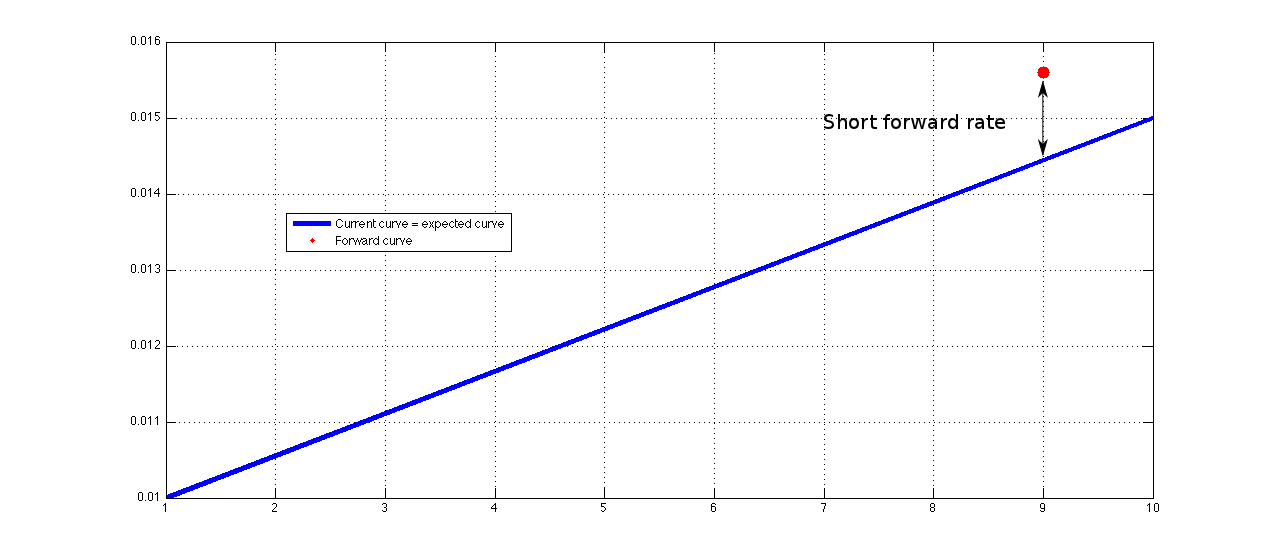
\includegraphics[width=5in] {pics/carry}
\caption{Carry trade when forward is different to current spot rate}
\label{fig:carry}
\end{figure}

We could get a very similar exposure by buying a properly priced bond future on the 10 year bond expiring in a year, or by buying a future on the the 9 year rate one year forward. All of these trades have the \textit{effect} of borrowing money at the low rate and lending it at the high rate.


\subsubsection*{Between curve carry:}

Rates differ across curves but also among curves.  A swap which pays a low rate and receives a high rate at the same maturity is also a carry trade. The $SW_{J1,S1}$ swap is an example. The swap pays the low Jesus rate and receives the high (and risky) Steve rate.

The swap has positive carry as a compensation for assuming the riskiness of the S1:

\[\frac{\partial V}{\partial t} = -y_{J1}*0.99*P_{J1}+y_{S1}P_{S1}= 0.9802 \]

Any other swap between curves with different yields can also be constructed with positive carry. The trick is to try to get the best carry for the least risk measured in spread duration, convexity, or whatever else you care about.


\subsubsection*{Cross currency carry:}

Rates differ between maturities and credit classes and also between countries. Riskless government bonds denominated in two currencies, will trade at different rates. Borrowing the cheap rate and lending the expensive rate is a carry trade.

The magic of arbitrage makes it unnecessary to actually borrow money in one country and lend it in another. The mechanics are bundled up into swaps and forwards. But the outcome is \textit{as if} you had borrowed and lent money. These can be used to convert loans in one currency to another or purely to extract the positive carry. We'll cover currency swap pricing in the next section so we won't go into it here but the basic idea is this: \textbf{if the low rate currency doesn't appreciate more than the interest rate difference the carry trade makes money}. 

\subsection{Rolldown trades}

Most yield curves are curvey, and some parts of the curve are curvier than others. Steep parts of the curve present an opportunity to a certain type of trader. If the curve retains its shape, the yield on a bond yield will \textbf{roll down} the curve, increasing the price of bond. The steeper the curve, the more pronounced the effect. Many fixed income strategies take advantage of this by positioning swaps and forwards on steep parts of the curve. We'll see in the example that this effect can be quite large, sometimes much larger than the pure carry, so it pays to be aware of rolldown even if you aren't trading it directly.

\begin{figure}[ht]
\centering
  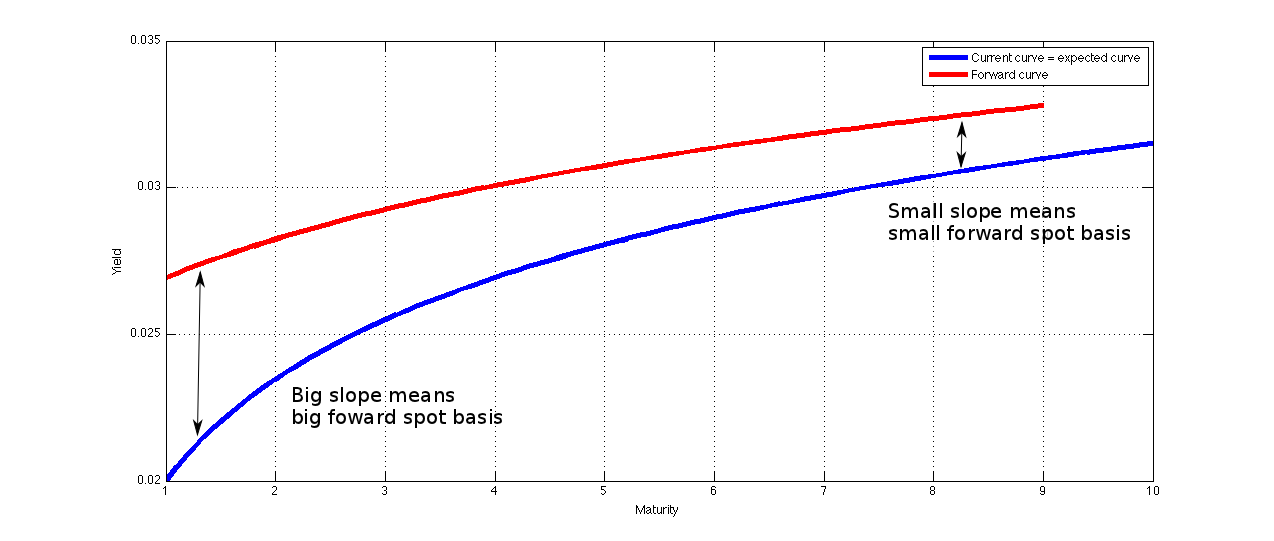
\includegraphics[width=5in] {pics/rolldown}
\caption{Rolldown trade on steep part of yield curve}
\label{fig:rolldown}
\end{figure}

%Example: y(T)  = @(T)(0.5*log(T)+2)/100;
%f = @(T2) (y(T2)*T2-y(1)*1)/(T2-T1)
%draw pic

The steeper the forward curve, the greater the difference between the forward rate and the spot rate, and so the greater the profit to the trade. Figure \ref{fig:rolldown} illustrates the effect on a convex yield curve: as the curve gets steeper the difference between forward and spot increases. 



One way to look at this is to decompose the value of a security into the yield and the rolldown. If we assume a constant slope $y(T)$ then the total yield is given the total derivative:

\[\frac{d V}{d t} = \underbrace{\frac{\partial V}{\partial y}\frac{\partial y}{\partial t}}_{\mbox{rolldown}} + \underbrace{\frac{\partial V}{\partial t}}_{\mbox{carry}}\ \]

It's similar with a swap whose value depends on a spread $S$ (which is a function of $y(T)$), then:

\[\frac{d V}{d t} = \underbrace{\frac{\partial V}{\partial S}\frac{\partial S}{\partial t}}_{\mbox{rolldown}} + \underbrace{\frac{\partial V}{\partial t}}_{\mbox{carry}}\ \]


\textbf{Example of a rolldown trade:}\\

We'll make a yield curve that is steep at the start and flattens out at longer maturities.\footnote{This one is $y(T) = (0.5*\ln(T)+2)/100$. In the real world yield curves don't have parametric forms but this makes the calculations easier.}  Table \ref{tab:rolldownTable} has the details. We proxy the slope of the spread curve $\frac{\partial S}{\partial t}$ by the slope of the chord connecting each adjacent spread. 

\[\mbox{Slope between $T_1$ and $T_2$} = \frac{\partial S}{\partial t} \approx \frac{y(0,T_2)-y(0,T_1)}{T_2-T_1} \]

This is an approximation but it's fine for our purposes.

\begin{center}
\begin{table}
\begin{tabular}{|c|cccccc|}
\hline
Maturity (years) & 1 & 2 & 5 & 6 & 10 & 11\\
Yield & 2\% & 2.34\% & 2.8\% & 2.90\%  & 3.15\% & 3.2\%\\  
1 year forward & & 2.69\% & 3.01\% & 3.08\% & 3.28\% & 3.32\% \\
spread to 1 year ($S$) & 0 & 0.34\% & 0.80\% & 0.90\% & 1.15\% & 1.2\%\\ 
$\frac{\partial S}{\partial t}$ & & -0.0034 & -0.0015 & -0.0009 & -0.0006 & -0.0005\\
\hline
\end{tabular}
\caption{Yields, forwards, spreads, and slopes}
\label{tab:rolldownTable}
\end{table}
\end{center}
%working in google docs 'working'


We know that we want to trade on the steep part of the curve, but we don't know exactly why yet. Everything becomes clear if we construct three swaps: $SW_{1,2}$, $SW_{1,6}$, and $SW_{1,11}$. (do this in the usual way, paying 1 year, receiving the longer maturity bond). The total yield is decomposed in table \ref{tab:decomposeSwap}:

\begin{center}
\begin{table}
\begin{tabular}{|c|cccccc|}
\hline
 & $\frac{\partial V}{\partial S}$ &$\frac{\partial S}{\partial t}$ & $\frac{\partial V}{\partial t}$ & $\frac{\partial V}{\partial S}\frac{\partial S}{\partial t}$ & $\frac{d V}{d t}$ & carry/rolldown\\
 \hline
$SW_{1,2}$ & -190.8 & -0.0034 & 0.331 & 0.661 & 0.992 & 0.5\\
$SW_{1,6}$ & -504.3 & -0.0009 & 0.753 & 0.460 & 1.213 & 1.64\\
$SW_{1,11}$ & -773.7&-0.0005 & 0.843 & 0.369 & 1.212 & 2.29\\
\hline
\end{tabular}
\caption{Decomposing swaps into carry and rolldown}
\label{tab:decomposeSwap}
\end{table}
\end{center}

Even though the $SW_{1,11}$ swap has a higher carry it has a lower expected total yield than the $SW_{1,6}$. Adjusted for spread duration ($\frac{\partial V}{\partial S}$) the $SW_{1,2}$ is clearly superior: it give a yield of around the same as the others with around a third the risk. The reason is that the effect of the additional carry gained from the higher yield of the 11 year bond is outmuscled by the rapidly declining yield of at the 1-2 year end of the curve. This is clear in the figure which shows the steep short end has the greatest difference between spot and forward rates. 

These kind of trades are wildly popular in fixed income funds, though often traders give more grand explanations. They are fairly persistently profitable, though still risky. A variant is to trade pairs with long positions on the steeper end of the curve and short positions on the flatter end. Another is to trade pairs across countries: long the steep curves and short the flat/inverted curves. The idea is to get the benefits of the rolldown while insulating the trade against global movements in yields. The exact implementation will depend as usual on risk preferences, liquidity, and such.

\subsection{Summary}

Carry trades borrow cheap money and lend expensive money. This can be done across a single yield curve or across different yield curves. Rolldown trades exploit an expectation that the curve will retain its shape by shorting the forward rate when the slope is large.


\textbf{Carry trades}:\\

\textit{Between curve carry}:\\

Enter a swap paying a low yield and receiving a high yield at different maturities.

\textit{Across curve carry}:\\

Enter a swap paying a low yield and receiving a high yield at the same maturity for two different borrowers.

\textit{Cross currency carry}:

Enter a swap to pay a low yield currency and receive a high yield currency at the same maturity.

\textbf{Rolldown trades}:

Enter a swap that is short the forward rate at a maturity where the curve is steep or long the forward rate when the curve is steeply negative.

\section{Currency and inflation}

We'll look at two swaps: a \textbf{cross currency swap} and an \textbf{inflation swap}. To construct these swaps we follow the same three step process we did for rates and credit:

\begin{enumerate}
\item Set a target exposure for the swap (e.g. the currency exchange rate)\\
\item Find two instruments which differ only in the target exposure (e.g. a bond from country A and a bond from country B at the same maturity)\\
\item Create a self financing (zero cost) portfolio by buying and short selling (paying and receiving) the two instruments\\
\end{enumerate}

And wallah! You've got your target swap. 

\subsection{A currency swap}

There are two countries: Australia and Barbados. Both issue 1 year bonds which are for the sake of the story are risk free. Australia issues in Australian dollars prefixed $\$A$, Barbados issues in Barbadian dollars prefixed $\$B$. Both bonds have a face value of 100 in the local currency. The exchange rate between the two countries is $X_{\$A,\$B}$, the number of Australian dollar for each Barbadian dollar. 

\begin{center}
\begin{tabular}{|c|ccc|}
\hline
 & Yield & Price & Exchange rate\\
 Australia 1 year bonds (A1) & 1\% & 99.01 & $X_{\$A,\$B}(0) = 0.5$\\
 Barbados 1 year bonds (B1) & 2\% &  98.01 &$X_{\$B,\$A}(0) = 2$\\
\hline
\end{tabular}
\end{center}
 
 The cost of a Barbados bond in Australian dollars is $98.01*0.5 = 49.01$. To purchase one Barbadian bond costs 49.01/99.01 = 0.495 Australian bonds. The self financing portfolio is short 0.495 Australian bonds and long 1 Barbados bond.
 
 \[V(0) = -0.495*P_{A1}(0) + P_{B1}(0)X_{\$A,\$B}(0) = 0 \]
 
 After one year both bonds mature and we pay \$A49.5 and receive \$B100. Exchange the \$B100 back at the prevailing exchange rate in 1 year and the total payoff is
 
 \[V(1) = -0.495*P_{A1}(1)+100*X_{\$A,\$B}(1) \]
 
The breakeven for this trade is when $X_{\$A,\$B}(1) = 0.495$ (see figure \ref{fig:currency}). If the exchange rate is greater the swap makes money. This means we can afford for the Australian dollar to drop 1\% against the current exchange rate and still make money. 
 
 The carry in Australian dollars is positive:
 
 \[\frac{\partial V}{\partial t} = -y_{A1}*0.495*P_{A1} + y_{B1}*P_{B1}*X_{A\$,B\$} (0)= 0.49 \]

The only uncertainty is the currency, so the currency swap is a pure linear exposure to the future exchange rate.

\begin{figure}[ht]
\centering
  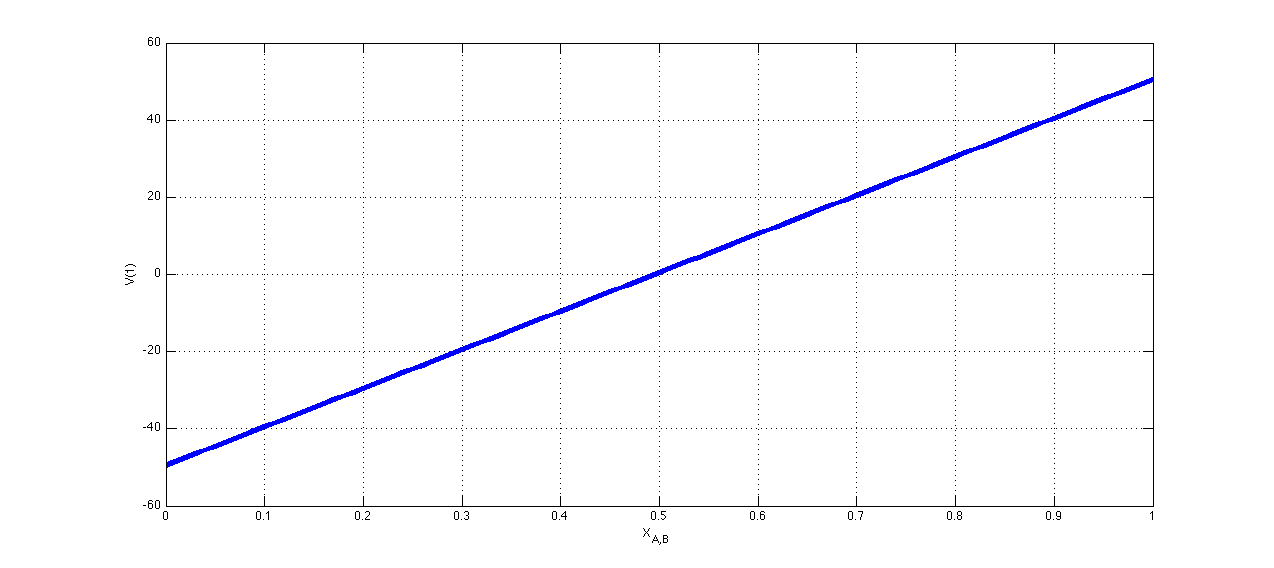
\includegraphics[width=5in] {pics/currency}
\caption{Currency swap payoff}
\label{fig:currency}
\end{figure}
 
\subsection{An inflation swap}

The problem with borrowing money from governments is that they have it in their power to create money to pay off their debts.  Printing money will lead to inflation, which means the money in the future is less valuable. Bond yields will account for this: borrowers will demand a higher yield to compensate for the loss of value in the currency at maturity. In many instances the quantum of this \textbf{inflation premium} is unobservable; it is mixed in with the real yield. However sometimes governments issue \textbf{inflation linked bonds} with a face value (and/or coupon) linked to a measure of inflation. These bonds can be stripped of the inflation component which prices separately as an \textbf{inflation swap}.

Inflation linked bonds come in a few flavours but here we'll take a zero coupon bond that repays $100*(1+I)$ at maturity where $I$ is the increase in some inflation measure (usually the Consumer Price Index).  A inflation linked bond and a normal bond trade at \$99.01 and \$99.5. 

\begin{center}
\begin{tabular}{|c|ccc|}
\hline
 & Yield & Price  & Face value \\
 \hline
1 year bonds (A1) & 1\% & 99.01 & 100 \\
1 year inflation linkers (I1) & ?\% &  99.5 & $100(1+I)$\\
\hline
\end{tabular}
\end{center}

We don't know what the yield of the linker is because we don't know what $I$ will be. We can however determine the market price of inflation by constructing a swap short 99.5/99.01 = 1.005 normal bonds and long one linker. 

The swap is self financing:

\[ V(0) = -1.005*P_{A1}(0) + P_{I1}(0) = 0\]

At expiry we have

\[ V(1) =  -1.005*100 + 100*(1+I)\]

This is a fixed for floating swap: the fixed rate is 1.005 and the floating rate is $(1+I)$. The swap is  a linear exposure to future inflation which breaks even when $I=0.005$. The market expects inflation to run at 0.5\% for the year. 

\begin{figure}[ht]
\centering
  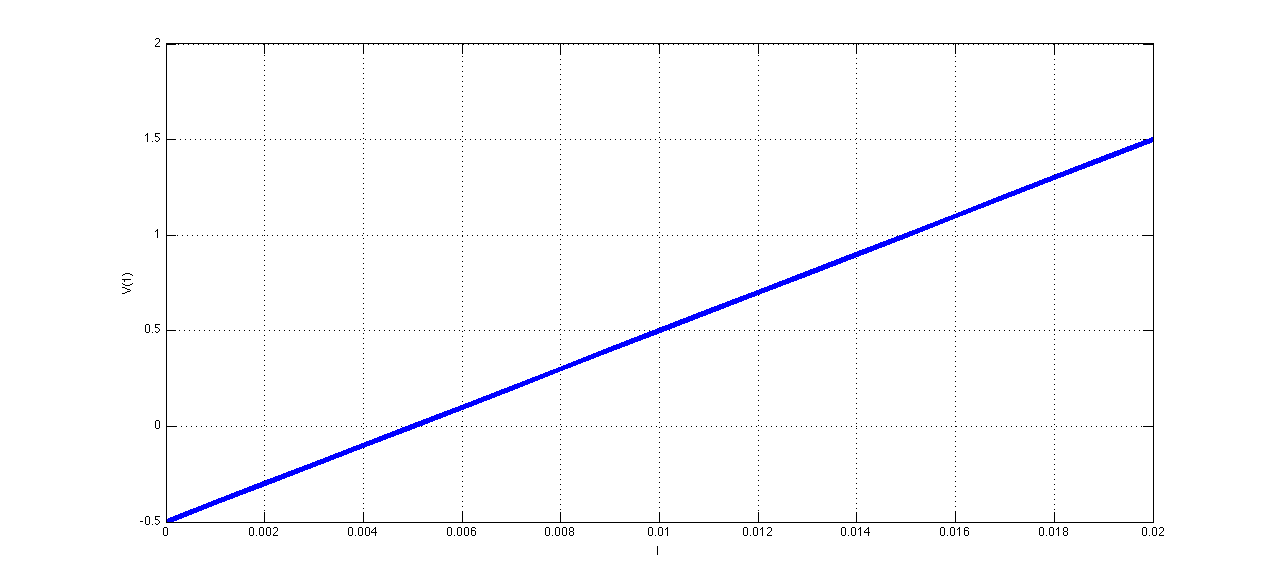
\includegraphics[width=5in] {pics/inflation}
\label{fig:inflation}
\caption{Inflation swap payoff}
\end{figure}

\subsection{Summary}

A currency swap pays and receives in two different currencies, an inflation swap pays a fixed face value and receives a face value dependent on the inflation rate.

\textbf{A currency swap}\\
Enter a fully financed swap paying a bond in currency $A$ and receiving a bond in currency $B$ at the same maturity. This gives an exposure to the forward exchange rate.

With arbitrary yields and maturity $T$ the swap has the following payoff in \$A:

\begin{eqnarray*}
V(T) = -\frac{P_{BT}(0)}{P_{AT}(0)}*P_{AT}(T)+ P_{BT}(T)*X_{\$A,\$B}(T) \\
 =  FV_A\exp((-y_{BT}+y_{AT})*T)+ FV_B*X_{\$A,\$B}(T)  
 \end{eqnarray*}

where $X$ is the exchange rate and $FV$ is the face value of the bonds. The only uncertain value is the future currency rate $X_{\$A,\$B}(T)$.

\textbf{An inflation swap}

Enter a swap to pay a normal bond $AT$ and receive an inflation linked bond $IT$ with the same maturity. The resulting exposure is the inflation linked portion of the linker. 

\begin{eqnarray*}
V(T) = \frac{P_{IT}(0)}{P_{AT}(0)}*P_{AT}(T)+ P_{IT}(T) \\
 =  FV\exp((-y_{IT}+y_{AT})*T)*P_{AT}(T)+ FV(1+I)  
 \end{eqnarray*}

The only uncertain value is the inflation rate $I$.


\section{Questions}

\textbf{Question 1:}\\
Consider the swap $SW_{J1,S10}$ from the credit and duration section. 

\begin{itemize}
\item[(a)] Give the equations for $V(0)$, $V(1)$
\item[(b)] Calculate the dollar yield and spread duration.
\item[(c)] Which interest rate is the swap exposed to? What is the breakeven?
\end{itemize}

\textbf{Question 2}\\

A client wants an annualised yield of \$5 and a spread duration of 0.03. Give the combination of $SW_{J1,J10}$s and $SW_{J10,S10}$s that will achieve this. What is the notional value of the exposure in terms of each underlying bond?

\textbf{Question 3:}\\

You expect that the yield curve in one year will be exactly 1\% higher than the one year forward curve. Construct a trade using $SW_{J1,J3}$ and $SW_{J1,J5}$ with equal DV01 to the forward rates to generate a payoff of \$10.

\textbf{Question 4:}\\

A yield curve is given by 

\[ y(T) = \frac{0.05\sqrt{T}+2}{100}\]

\begin{itemize}
\item[(a)] Derive the 5 year forward curve
\item[(b)] Generate an expression for the total yield of a generic swap $\frac{d V_{SW_{T_1,T_2} } }{d t}$ including the carry and rolldown. %del V \ del t del spread del t
\end{itemize}

\textbf{Question 5:}\\

You expect a payment of 10 Barbados dollars in one year. What is the annualised yield of the swap to hedge this into Australian dollars? 




%\subsection{A sovereign default swap}

%Normally government debt is considered risk free. All other debt prices at a spread and we construct a CDS by shorting government against more risky bonds.  However sometimes governments do default. And even if they don't the possibility that they might in future is incorporated into the yield. Credit default swaps trade on sovereign debt in much the same way they do on corporate debt. But there are some troubles.

%The main trouble is that it's difficult to construct an arbitrage portfolio for a credit default swap on government debt (a \textbf{sovereign default swap}) because there's no risk free borrower for the other side of the trade. It's possible to finance the trade with a more or less risky borrower, but then the swap is a \textbf{joint default swap}. If other bonds are issued by a risk free borrower in the same currency then there is no problem: we can construct a sovereign CDS as we would a normal CDS: long the risky bond, short the risk-free bond.









 
